%% ==========================================================================
%%  AAAI-27 submission (FULL DRAFT FRAMEWORK) — Personal Fact Memory (PFM)
%%  DOUBLE-BLIND / ANONYMIZED for review.
%%
%%  This file is the complete paper skeleton with all sections written out.
%%  Unfinished content is marked with \todo{...} (renders in red).
%%  Search for "TODO" to find every placeholder before submission.
%%
%%  BEFORE COMPILING you MUST download the AAAI-27 Author Kit and place
%%  these files next to this .tex (the kit is the ONLY authoritative source):
%%      aaai27.sty      aaai27.bst
%%  Get it from: https://aaai.org/conference/aaai/aaai-27/  (Author Kit link).
%%
%%  Compile:  pdflatex -> bibtex -> pdflatex -> pdflatex
%%            (bibliography file: aaai2027.bib, in this folder)
%%
%%  HARD RULES from the AAAI kit (do NOT change / do NOT add):
%%    - No \usepackage{hyperref}       (AAAI forbids it in submissions)
%%    - No geometry / fullpage / authblk / titlesec / etc. margin packages
%%    - US Letter, two-column, Type 1 fonts (times/helvet/courier)
%%    - Main PDF <= 9 pages; pages 8-9 references ONLY; <= 7 content pages
%%    - Remove ALL author/affiliation identity for review (done below)
%%
%%  数字来源（正文所有实验数字与下列文档逐一核对过，改动前先改源头）：
%%    ../8_dpfm_application/docs/DPFM-EXPERIMENT-REPORT.md   (Study 1)
%%    ../8_dpfm_application/docs/dpfm-parameter-design.csv   (参数表)
%%  投稿前删除：xcolor + \todo 宏（连同所有占位符）。
%% ==========================================================================

\documentclass[letterpaper]{article}

\usepackage{aaai27}          % from the AAAI-27 Author Kit
\usepackage{times}           % roman text font
\usepackage{helvet}          % sans-serif font
\usepackage{courier}         % typewriter font
\usepackage[hyphens]{url}    % url breaking
\usepackage{graphicx}        % figures
\urlstyle{rm}
\def\UrlFont{\rm}
\usepackage{natbib}
\usepackage{caption}
\frenchspacing
\setlength{\pdfpagewidth}{8.5in}
\setlength{\pdfpageheight}{11in}

% --- Extra math/table packages that ARE allowed by the kit ---------------
\usepackage{amsmath}
\usepackage{amssymb}
\usepackage{booktabs}
\usepackage{algorithm}
\usepackage{algorithmic}

% --- DRAFT ONLY: placeholder machinery. REMOVE before submission. --------
\usepackage{xcolor}
\newcommand{\todo}[1]{\textbf{\textcolor{red}{[TODO: #1]}}}
\newcommand{\figplaceholder}[2]{%
  \fbox{\parbox[c][#1][c]{0.94\columnwidth}{\centering\todo{#2}}}}

% --- Notation shortcuts ---------------------------------------------------
\newcommand{\Du}{D_u}
\newcommand{\deadline}{\Delta}
\newcommand{\factset}{F}

% --- PDF metadata (required by the kit) ----------------------------------
\pdfinfo{
/TemplateVersion (2027.1)
}

\setcounter{secnumdepth}{0} % AAAI style: no section numbering

% ==========================================================================
\title{Personal Fact Memory: A Cognitively-Grounded, Latency-Bounded\\
       Memory Layer for On-Device LLM Assistants}

% --- DOUBLE-BLIND: no author identity during review. ---------------------
\author{
    Anonymous Submission
}
\affiliations{
    Paper ID: (assigned by OpenReview)
}
% ==========================================================================

\begin{document}
\maketitle

\begin{abstract}
Persistent memory for an on-device language assistant must satisfy three
constraints jointly: retrieved facts must concern the intended person, remain
valid as personal information changes, and arrive before generation commits
to a response. We formulate this as \emph{deadline-constrained personal fact
retrieval}: returning a small set of currently valid, identity-correct facts
from an evolving personal store within a fixed serving deadline and memory
budget. Existing agent-memory systems address temporal consistency,
personalization, and retrieval efficiency separately, and assume server-scale
infrastructure an on-device assistant cannot afford. We
introduce Personal Fact Memory (PFM), which represents atomic facts in a
bitemporal entity graph where superseding values close their predecessors
instead of competing with them, and retrieves by bounded in-memory lexical
search with local graph expansion; no embedding model or LLM is invoked on
the hot path, and speculative prefetch with deadline racing makes retrieval
non-blocking by construction. Forgetting is biologically grounded: a dual
recency/usage-reinforcement decay---echoing the Ebbinghaus curve and the
testing effect---lets facts fade unless reinforced by accepted completions,
stratifies episodic, semantic, and pinned profile memory, and bounds the
store by use rather than corpus size. We further propose a choice-theoretic
serving layer: completion acceptance as discrete user choice, per-user fusion
weights estimated online from implicit accept/reject feedback, and
prompt-slot allocation under a character budget as constrained assortment
optimization. In offline replay from a deployed autocomplete assistant, PFM
raises ground-truth fact availability from 0\% to 96\% (24/25 scenarios) and
sustains 1.8~ms median retrieval at 20{,}000 facts---two orders of magnitude
below LLM prefill. PFM treats stale, misattributed, and late facts as
distinct failures, and the individual, not the corpus, as the unit of design.
\end{abstract}

% Keywords (OpenReview form field only; AAAI main track prints none):
% Personalized Memory Systems; On-Device LLM Agents; Cognitively-Inspired
% Memory Architecture; Low-Latency Retrieval-Augmented Generation; Bi-Temporal
% Knowledge Representation; Discrete Choice Models; Assortment Optimization;
% Real-Time Text Completion

% ==========================================================================
\section{Introduction}
% 故事线：GUI 场景开场 → 端侧转移 → 三约束 → 现有系统合起来都不满足 →
% PFM → 贡献清单。Fig.1 是 teaser（GUI 截图 + memory block 注入示意）。
% ==========================================================================

Consider a user typing an email in an ordinary desktop application. A
system-wide autocomplete assistant watches the text field and offers an
inline, greyed-out continuation---\emph{ghost text}---that the user can
accept with a single keystroke (Figure~\ref{fig:teaser}). The user types ``The Phoenix deadline
is''\,; a useful continuation is not fluent prose but a \emph{fact}: the
correct date, for the correct project, as most recently revised, copied
verbatim. If the assistant's language model has never seen the user's past
messages, it can only guess. If a memory layer supplies the wrong person's
deadline, a superseded date, or arrives after the model has already
committed to a token, the completion is worse than none: it is confidently
wrong inside the user's own sentence.

\begin{figure}[t]
\centering
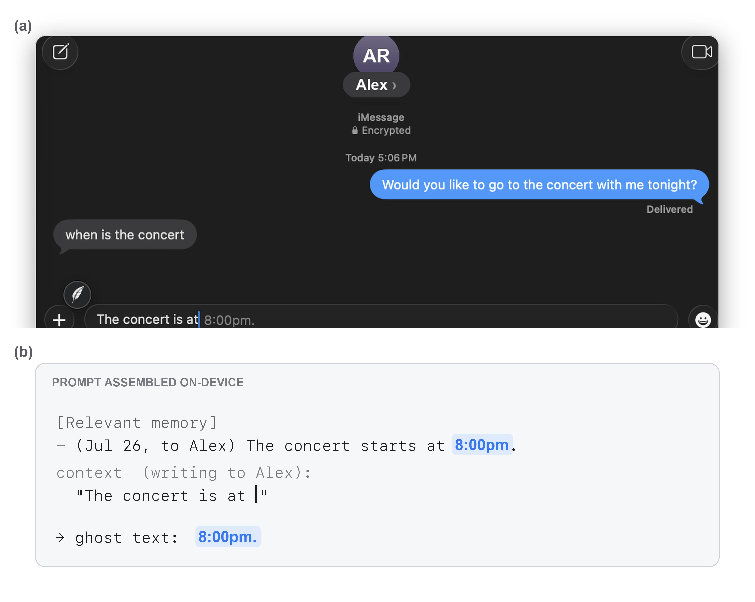
\includegraphics[width=\columnwidth]{figures/teaser.pdf}
\caption{PFM in the deployed assistant (recipient pseudonymized).
\textbf{(a)}~As the user replies to ``when is the concert,'' the assistant
completes ``The concert is at'' with inline ghost text \texttt{8:00pm.}
\textbf{(b)}~The completion is not a guess: the memory layer injected a
small, budgeted \texttt{[Relevant memory]} block into the (frozen) model's
prompt, letting it copy the remembered time verbatim. Accepting a
completion feeds back into the memory layer, reinforcing the facts that
produced it.}
\label{fig:teaser}
\end{figure}

This scenario is no longer hypothetical. Small language models in the
7--9B range now run with acceptable interactive quality on consumer
hardware, and privacy expectations push personal assistants toward local
deployment. What is missing is not the model but its
\emph{infrastructure}: a persistent memory of the user's own facts that the
model can consult on every request. We argue that such a memory layer faces
three constraints that must hold \emph{jointly}, and that each corresponds
to a distinct, observable failure mode:

\begin{itemize}
\item \textbf{Identity.} Retrieved facts must concern the intended person
  and entities. Failure: a \emph{misattributed} fact---another contact's
  deadline surfaced because the sentence is lexically similar.
\item \textbf{Validity.} Personal information is constantly revised
  (addresses, meeting times, budgets); the newest value must supersede,
  not coexist with, its predecessors. Failure: a \emph{stale} fact.
\item \textbf{Deadline.} Autocomplete fires on keystrokes; retrieval that
  arrives after the host model begins prefill is useless and retrieval
  that blocks it degrades the product it serves. Failure: a \emph{late}
  fact.
\end{itemize}

Existing LLM agent-memory systems address these concerns separately, and
under assumptions that an on-device assistant cannot meet. Their write and
read paths rely on embedding models and LLM calls---an unacceptable extra
forward pass when the local model is already the scarce resource---and
their evaluations report QA accuracy on server-scale benchmarks rather
than millisecond latency under a serving deadline (see Related Work).
The most cognitively sophisticated of them explicitly assumes centralized
deployment~\citep{kerestecioglu2026human}. The most recent
survey~\citep{du2026survey} lists memory-efficient architectures and
deeper neuroscience integration as \emph{separate} open problems and
never connects either to single-user personalization.

We introduce \textbf{Personal Fact Memory (PFM)}, a memory layer designed
for exactly this joint constraint, instantiated in a commercially deployed
macOS autocomplete assistant (name withheld for review). PFM rests on
three pillars: (P1) \emph{identity-grounded association}---atomic facts
carry entity and participant attribution, retrieval scores participants
above generic text, and contradictory slot values are closed bitemporally
rather than left to compete; (P2) \emph{bounded-footprint, deadline-safe
serving}---a pure in-memory lexical hot path with speculative prefetch and
deadline racing that is non-blocking by construction (Proposition~1); and
(P3) \emph{biologically-grounded stratification}---episodic, semantic, and
pinned profile facts decay under a dual recency/usage-reinforcement
schedule that echoes the Ebbinghaus forgetting
curve~\citep{ebbinghaus1885memory} and the testing
effect~\citep{roediger2006test}. On top of the architecture we propose a
\emph{choice-theoretic serving layer}: treating completion acceptance as a
discrete choice~\citep{mcfadden1974conditional} whose implicit
accept/reject feedback estimates per-user fusion weights online, and
treating prompt-slot allocation under a character budget as constrained
assortment optimization~\citep{talluri2004revenue,
rusmevichientong2010dynamic}.

Our contributions are:
\begin{enumerate}
\item A formulation of \emph{deadline-constrained personal fact retrieval}
  with a failure typology (stale, misattributed, late) that makes the
  joint constraint of on-device personal memory explicit and measurable.
\item The PFM architecture (P1--P3), including a provable non-blocking
  serving guarantee and a use-bounded forgetting policy, with no
  embedding or LLM call on the hot path.
\item A choice-theoretic serving layer that turns implicit accept/reject
  feedback into per-user, interpretable retrieval parameters and casts
  prompt injection as budgeted assortment optimization---with the
  facts$\rightarrow$completion$\rightarrow$acceptance mediation stated as
  an explicit modeling assumption.
\item Deployment and evidence: an offline replay study from the deployed
  assistant showing ground-truth fact availability rising from 0\% to
  96\% (24/25 scenarios) against ${\sim}270$ competing facts, with
  0.011~ms median retrieval at deployed scale and 1.81~ms at 20{,}000
  facts---two orders of magnitude below LLM prefill. Ablations isolate
  the pillars: identity probes fall from 8/8 to 5/8 without the
  participant field (Study~4), and in simulation the assortment layer
  matches the deployed baseline's acceptance within 3 points on 17\%
  fewer injected characters under a binding budget (Study~3). The live
  in-app A/B (Study~2) remains protocol-only.
\end{enumerate}

% ==========================================================================
\section{Related Work}
% 四段 + 对照表：agent memory 系统 / 认知启发架构 / 端侧与评测 / OR 工具。
% 结尾一段是 gap 陈述（从 1_gap_analysis.md §2 直译）。
% ==========================================================================

\paragraph{LLM agent memory systems.}
Mem0 structures writing as a two-phase extract--update pipeline with
LLM-arbitrated ADD/UPDATE/DELETE decisions~\citep{chhikara2025mem0};
Zep/Graphiti maintains a temporal knowledge graph whose bitemporal edges
invalidate rather than delete superseded facts~\citep{rasmussen2025zep};
HippoRAG performs associative multi-hop recall over an entity graph with
Personalized PageRank~\citep{gutierrez2024hipporag}; MemoryOS manages
heat-driven hierarchical promotion and eviction~\citep{memoryos2025};
A-MEM builds Zettelkasten-style atomic notes with automatic
linking~\citep{xu2025amem}; MemGPT/Letta pages between core and archival
memory tiers~\citep{packer2023memgpt}; MemoryBank applies
Ebbinghaus-style decay to conversational summaries~\citep{zhong2023memorybank}.
PFM borrows one mechanism from each (the mapping is made explicit in the
Architecture section) but differs in \emph{who} the machinery serves: in
all of these systems, identity is a routing key or one node among many.
None weights participant attribution as a first-class retrieval field, and
none treats ``the newest value must overwrite its predecessor in the
prompt'' as a core requirement of the personal setting. Their evaluations
target multi-user or open-domain QA benchmarks such as
LOCOMO~\citep{maharana2024evaluating} and
LongMemEval~\citep{wu2024longmemeval}, reporting accuracy but not
end-to-end latency under a serving deadline.

\paragraph{Cognitively grounded memory architectures.}
A growing 2026 line grounds agent memory in cognitive science. The
Human-Inspired Memory Architecture~\citep{kerestecioglu2026human} is the
most complete: complementary learning systems, sleep-time consolidation,
Ebbinghaus decay with interference, engram maturation, and
reconsolidation. Yet it explicitly assumes centralized deployment
(GPT-4o + \texttt{text-embedding-3-large}), and its authors acknowledge
that the two most biological mechanisms---engram maturation and
reconsolidation---remain \emph{empirically unvalidated} because QA
benchmarks never accumulate repeated-access signals. Concurrent work
applies the Ebbinghaus curve to long-context
compression~\citep{icict2026ebbinghaus} and proposes multi-layer
neurocognitive architectures~\citep{zenbrain2026}, neither under edge
constraints. We observe that the personal-assistant setting
\emph{naturally provides} the missing repeated-access signal---the same
user repeatedly triggers, accepts, and rejects completions---and PFM's
usage-reinforcement term is a deployable, measured simplification of the
reconsolidation hypothesis those systems could not test.

\paragraph{On-device personalization and evaluation readiness.}
EdgeTune personalizes by on-device LoRA adaptation~\citep{edgetune2026},
which is orthogonal to a queryable external memory: tuning changes what
the model \emph{is}, not what it can \emph{look up}, and cannot copy a
revised deadline verbatim. \citet{zhou2026ready} question whether current
memory systems are production-ready and elevate latency and storage
footprint to first-class evaluation dimensions---a call for exactly the
kind of measured, deadline-constrained system we present, but without
providing one.

\paragraph{Discrete choice and assortment optimization.}
Our serving layer imports two classical tools from econometrics and
revenue management: the conditional (multinomial) logit model of
choice~\citep{mcfadden1974conditional}, and assortment optimization under
MNL demand, where revenue-ordered assortments are optimal in the
unconstrained case~\citep{talluri2004revenue}, cardinality constraints
admit polynomial algorithms~\citep{rusmevichientong2010dynamic}, and
knapsack-type constraints admit an FPTAS~\citep{desir2020capacitated}.
In LLM research, choice models have recently entered on the
\emph{training} side: RCPO generalizes DPO~\citep{rafailov2023direct} and
SimPO~\citep{meng2024simpo} with ranked-choice objectives, updating model
weights from curated preference data~\citep{tang2026rcpo}. We use the same
statistical family on the \emph{serving} side: the LLM is frozen, the data
are implicit binary accept/reject events from real use, and the object
optimized is five interpretable scalars per user plus one combinatorial
injection decision per request.

\paragraph{The gap.}
\emph{Existing systems either optimize retrieval accuracy for
generic/multi-user settings, or go deeper on cognitive alignment while
assuming server-scale infrastructure, unbounded latency, and benchmarks
that cannot validate their biological mechanisms. No prior work treats
single-user identity grounding, millisecond-deadline/bounded-storage
serving, and biologically stratified forgetting as one joint design
constraint---the two open problems the latest survey lists separately and
never connects~\citep{du2026survey}---nor reports deployment-grade
measurements under that constraint.} Table~\ref{tab:comparison}
summarizes.

\begin{table}[t]
\centering
\small
\begin{tabular}{@{}lcccc@{}}
\toprule
System & Identity & Deadline & Cognitive & Deployed \\
\midrule
Mem0                & \(\circ\) & --        & --        & \(\bullet\) \\
Zep/Graphiti        & \(\circ\) & --        & --        & \(\bullet\) \\
HippoRAG            & --        & --        & \(\circ\) & --          \\
MemoryOS            & --        & --        & \(\circ\) & --          \\
A-MEM               & --        & --        & --        & --          \\
MemGPT/Letta        & \(\circ\) & --        & \(\circ\) & \(\bullet\) \\
HIMA                & --        & --        & \(\bullet\) & --        \\
\midrule
\textbf{PFM (ours)} & \(\bullet\) & \(\bullet\) & \(\bullet\) & \(\bullet\) \\
\bottomrule
\end{tabular}
\caption{Coverage of the joint constraint.
\(\bullet\)~= first-class design target with evidence;
\(\circ\)~= partial/incidental; --~= absent.
\emph{Identity}: participant-aware retrieval with slot supersession.
\emph{Deadline}: non-blocking serving under a millisecond budget without
embedding/LLM calls on the hot path. \emph{Cognitive}: mechanisms mapped
to named memory science. \emph{Deployed}: measurements from a real
production integration. HIMA = Human-Inspired Memory
Architecture~\citep{kerestecioglu2026human}. PFM's Identity and Deadline
claims are measured directly by the identity-probe ablation of
Table~\ref{tab:ablation} and the latency results of
Tables~\ref{tab:latency} and~\ref{tab:ablation}.
\todo{Re-verify the prior-work cells against the cited papers before
submission.}}
\label{tab:comparison}
\end{table}

% ==========================================================================
\section{Problem Formulation}
% 2_framework_design.md §1 的直译 + 失败类型学。
% ==========================================================================

Let $u$ be a single user with a growing personal corpus
$\Du = \{d_1, d_2, \dots\}$ of documents the user has written or
received (messages, emails, notes), arriving as a stream. A completion
request supplies a typing context $c$ (the text around the cursor), a
participant set $P(c)$ (e.g., the recipient of the message being
written), and a serving deadline $\deadline$ set by the host model's own
prefill/network latency, typically 10--50~ms.

\begin{quote}
\textbf{Deadline-constrained personal fact retrieval.} Return
$\factset \subseteq \mathrm{Facts}(\Du)$ with $|\factset| \le k$ and
$\sum_{f \in \factset} \mathrm{len}(f) \le B$ characters, such that:
\begin{itemize}
\item[(a)] \emph{Identity grounding.} Each $f \in \factset$ carries its
  entity and participant attribution in $\Du$, and scoring weights
  attribution to the people/entities in $c$ and $P(c)$ above generic
  textual similarity, so that identically worded facts about different
  people are correctly separated.
\item[(b)] \emph{Deadline safety.} Retrieval completes within $\deadline$
  with high probability, and its cost degrades at most sublinearly in
  $|\Du|$---a personal corpus grows without bound, and a memory layer
  that slows down with age fails its product.
\item[(c)] \emph{Bounded footprint.} $|\mathrm{Facts}(\Du)|$ is bounded by
  a forgetting policy that adapts to usage rather than corpus size, while
  guaranteeing that pinned high-value facts (e.g., the user's own profile)
  are never evicted.
\item[(d)] \emph{Self-correction.} Contradictory updates to the same slot
  (e.g., \texttt{(phoenix, deadline)}) supersede: the old fact leaves the
  ranking (retaining an audit trail) so contradictions never co-occur in
  the injected prompt.
\end{itemize}
\end{quote}

Violating (a) yields \emph{misattributed} facts, violating (d) yields
\emph{stale} facts, and violating (b) yields \emph{late} facts---the three
failure modes of the Introduction. Property (c) is what makes (b)
sustainable over years of use. We deliberately do not fold these into a
single accuracy number: each failure is observable in deployment and each
pillar of the architecture answers one of them.

% ==========================================================================
\section{The Personal Fact Memory Architecture}
% 三支柱。Fig.2 = pipeline 图（2_framework_design.md §3 的 ASCII 图重画）。
% ==========================================================================

\begin{figure*}[t]
\centering
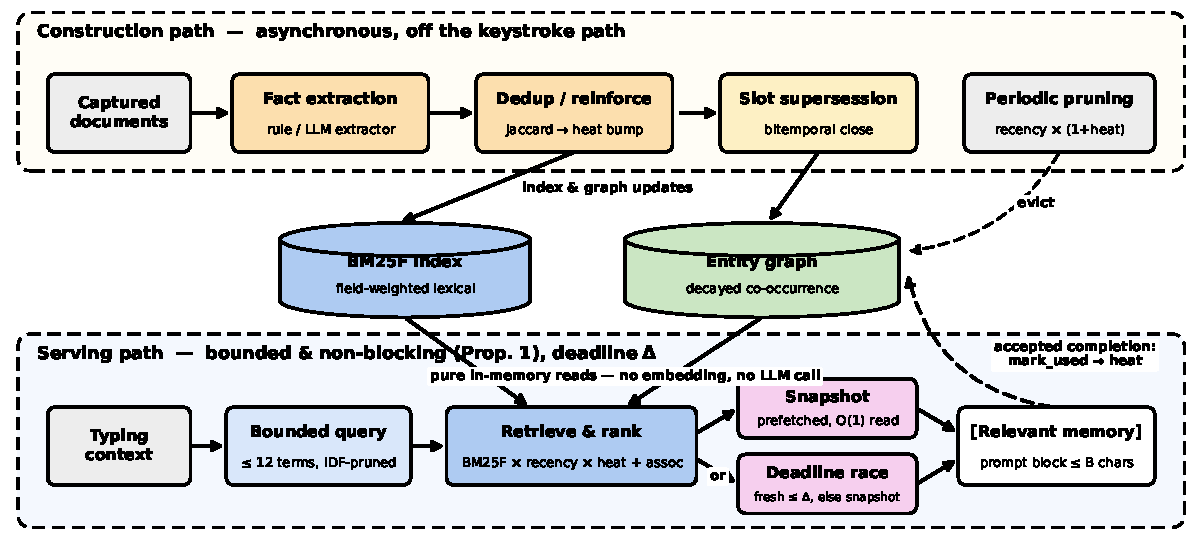
\includegraphics[width=0.96\textwidth]{figures/pipeline.pdf}
\caption{PFM separates asynchronous memory construction from retrieval at
completion time. The construction path extracts and updates facts,
maintains the lexical index and entity graph, and prunes stored state.
The serving path constructs a bounded query, retrieves and ranks active
facts, and supplies a prompt block through either a published snapshot or
a fresh retrieval with a fixed waiting budget.}
\label{fig:pipeline}
\end{figure*}

\subsection{P1: Identity-Grounded Association}

\paragraph{Atomic facts.}
The unit of memory is not a passage but an atomic, prompt-ready fact
\[
f = (\mathrm{text},\, E_f,\, P_f,\, \mathrm{kind},\, \mathrm{key},\,
     t_{\mathrm{from}},\, t_{\mathrm{inv}}),
\]
where $E_f$ are normalized entities, $P_f$ are the participants
(recipients/interlocutors) of the source document,
$\mathrm{kind} \in \{\text{episodic}, \text{semantic}, \text{profile}\}$,
$\mathrm{key}$ is an optional slot identifier, and
$(t_{\mathrm{from}}, t_{\mathrm{inv}})$ are bitemporal validity bounds.

\paragraph{Field-weighted lexical retrieval.}
Retrieval uses simple-BM25F~\citep{robertson2004simple,
robertson2009probabilistic} over three fields with weights
$\mathrm{text}{:}\,E_f{:}\,P_f = 1.0{:}\,2.5{:}\,2.0$. The choice of
lexical over semantic matching is a claim, not a shortcut: completion must
copy names, dates, and amounts \emph{verbatim}, so exact lexical evidence
is the right relevance signal, and the participant field---\emph{who this
document was written to}---is a strong personal-relevance feature that
generic semantic retrieval has no analogue for. This is the mechanism that
separates identically worded facts about different people: ``deadline
moved to Friday'' written to Alice and to Bob are lexically identical in
text but disjoint in participants. An optional embedding channel can be
fused by reciprocal rank fusion~\citep{cormack2009reciprocal} on the
prefetch path only; the system is fully functional without it.

\paragraph{Bitemporal slot supersession.}
When a new fact shares a $\mathrm{key}$ with an existing one, the old fact
receives $t_{\mathrm{inv}}$ and leaves the index without being destroyed
---adapting Zep's bitemporal edges~\citep{rasmussen2025zep} from
knowledge-graph consistency to the personal requirement (d): the prompt
must contain the current deadline, and only the current deadline, while
the audit trail survives.

\paragraph{Associative recall.}
An entity co-occurrence graph with decaying edge weights supports
truncated one-hop spreading activation---an $O(|\mathrm{seeds}| \times
\mathrm{degree})$ approximation of HippoRAG's Personalized
PageRank~\citep{gutierrez2024hipporag}. Where HippoRAG seeds propagation
from query terms for open-domain QA, PFM's seeds always come from the
\emph{same user's} identity graph: mentioning Alice recalls the Phoenix
project she runs even when the context never names it. Personalization is
not a parameter of the walk; it is the graph itself.

\subsection{P2: Bounded-Footprint, Deadline-Safe Serving}

\paragraph{Cold/hot path separation.}
Everything model-dependent or unbounded---extraction, deduplication,
graph updates, pruning---runs asynchronously on the cold path with no
latency ceiling. The hot path is pure in-memory computation:
query construction takes the tokens in a window before the cursor,
weights them by positional decay ($\lambda^d$, $\lambda{=}0.95$, nearer
the cursor is heavier), boosts participant terms ($+1.5$), and prunes to
at most 12 terms by $\mathrm{weight} \times \mathrm{idf}$ in the spirit of
WAND~\citep{broder2003efficient}---bounding posting-list work
regardless of context length. Term-at-a-time accumulation over
personal-scale posting lists ($10^3$--$10^5$ facts) plus a heap top-$k$
completes retrieval; no vector index, ANN search, embedding call, or LLM
call exists on this path.

\paragraph{Non-blocking serving.}
Two mechanisms make the memory layer unable to slow its host:
(i)~\emph{speculative prefetch}: a background thread retrieves during
typing pauses and publishes an immutable snapshot by atomic swap; a
completion request reads the current snapshot in $O(1)$;
(ii)~\emph{deadline race}: optionally, a fresh retrieval races the host
model's own budget $\deadline$ and falls back to the latest snapshot
(marked stale) on timeout.

\begin{quote}
\textbf{Proposition 1 (non-blocking by construction).}
% (手工编号；若改用 amsthm 的 proposition 环境需先确认 AAAI kit 兼容)
Let $r$ be the cost of one atomic snapshot read. In snapshot mode, the
worst-case latency PFM adds to the generation path is $r$; in deadline
mode it is at most $\deadline + r$. Neither bound depends on $|\Du|$, the
extractor, or any cold-path state.
\emph{Proof sketch.} Snapshots are immutable and published by a single
atomic pointer swap; the hot path takes no locks shared with the cold
path, so a read completes in $r$ regardless of concurrent writes. The
deadline race returns the fresh result if it arrives within $\deadline$
and otherwise the snapshot, so its latency is capped by the race timer
plus one read. $\square$
\todo{Write out the full proof (memory-model assumptions, latest-wins
debounce) in the technical appendix.}
\end{quote}

\paragraph{Use-bounded forgetting.}
Periodic pruning evicts facts with
$\mathrm{recency}(f) \times (1 + \mathrm{heat}(f))$ below threshold
(profile facts exempt) and prunes the graph accordingly. The store is
thereby bounded by \emph{usage}---which facts the user keeps touching---%
rather than by raw document volume, satisfying (c) and keeping hot-path
posting lists short, which is what sustains (b) as the corpus ages.

\subsection{P3: Biologically-Grounded Stratification}

\paragraph{Three strata.}
The $\mathrm{kind}$ field maps the fact store onto complementary learning
systems theory~\citep{mcclelland1995complementary}: \emph{episodic} facts
(hippocampal fast encoding) bind to a single source document and decay
with time and disuse; \emph{semantic} facts (neocortical slow
consolidation) are distilled from repeated observation and decay more
slowly; \emph{profile} facts (core self-schema) are pinned and never
forgotten.

\paragraph{Dual-decay scoring.}
The retrieval score fuses lexical evidence with two decay processes and
graph association:
\begin{equation}
\label{eq:score}
\begin{split}
\mathrm{score}(f) ={}& \mathrm{BM25F}(q,f) \cdot
  \Big(\varepsilon + (1-\varepsilon)\, 2^{-\Delta t / T_{\mathrm{rec}}}\Big)\\
&\cdot \big(1 + \eta \cdot \mathrm{heat}(f)\big)
  \;+\; \gamma \cdot \mathrm{assoc}(f).
\end{split}
\end{equation}
The recency term is an exponential forgetting curve with a nonzero floor
$\varepsilon$: old memories become hard to retrieve yet remain reachable
under a strong cue, mirroring Ebbinghaus's savings
effect~\citep{ebbinghaus1885memory}. The heat term is a decaying counter
incremented when the user \emph{accepts} a completion built from $f$
(\texttt{mark\_used}): retrieval-that-leads-to-use strengthens the trace,
mirroring the testing effect~\citep{roediger2006test} and closing the
loop in Figure~\ref{fig:pipeline}. The result is a memory that ``fades
unless used,'' with usage defined by the product's own acceptance signal
rather than by an artificial rehearsal schedule.

\paragraph{Relation to unvalidated reconsolidation mechanisms.}
\citet{kerestecioglu2026human} could not validate engram maturation or
reconsolidation because their benchmarks never revisit a memory. PFM's
heat mechanism is a running, measured simplification of exactly that
hypothesis---repeated retrieval-and-acceptance reconsolidates the
trace---in the one setting that naturally generates the required signal.
We do not claim biological fidelity; we claim that the personal-assistant
loop is the right test bed for this family of mechanisms, and we provide
the first deployment-grade instance.

% ==========================================================================
\section{Choice-Theoretic Memory Serving}
% 2_framework_design.md §4。诚实标注：提案 + Study 3 验证（占位）。
% 若 7/28 前 Study 3 没跑完：本节保留，但贡献列表与摘要维持 "propose" 措辞。
% ==========================================================================

The architecture above leaves two gaps. First, the fusion parameters in
Eq.~\eqref{eq:score}---$\varepsilon, \eta, \gamma, T_{\mathrm{rec}},
T_{\mathrm{heat}}$---are global constants: personalization lives in the
corpus but not in the retrieval function itself. Second, the final
injection decision is top-$k$ by score with greedy truncation, which is
suboptimal under substitution: two high-scoring near-duplicates cannibalize
each other's contribution while consuming two slots of the character
budget. We address the first with a discrete choice model and the second
with constrained assortment optimization.

\subsection{Demand Side: Acceptance as Discrete Choice}

Every completion request that injects a fact set $S$ ends in an observable
binary outcome: the user accepts (triggering \texttt{mark\_used}) or
implicitly rejects. We model this as a discrete choice with an outside
option~\citep{mcfadden1974conditional}. Each fact carries a log-linear
attraction
\begin{equation}
\label{eq:utility}
w_f = \exp\!\big(\theta^{\top} x_f\big), \quad
x_f = \big(\log \mathrm{BM25F},\, \Delta t,\, \mathrm{heat},\,
\mathrm{assoc}, 1\big),
\end{equation}
and the acceptance probability of an injected set is
\begin{equation}
\label{eq:mnl}
\Pr[\text{accept} \mid S] \;=\;
\frac{\sum_{f \in S} w_f}{1 + \sum_{f \in S} w_f}.
\end{equation}
The per-user parameter vector $\theta_u$ is estimated by online maximum
likelihood---single SGD steps on the log-likelihood of each sparse
accept/reject observation, executed on the cold path so the hot path is
untouched. Beyond accuracy, $\theta_u$ is an interpretable
\emph{individual profile}: a high heat coefficient describes a user who
relies on repetition-reinforced facts; a high association coefficient, a
user whose contexts under-specify entities and lean on graph recall.
Individual difference becomes a measured output of the system, not only a
design goal.

\emph{Positioning.} RCPO~\citep{tang2026rcpo} applies ranked-choice models
on the training side, generalizing DPO/SimPO objectives over curated
preference data to update LLM weights. We share only the statistical
family: here the LLM is frozen, the data are implicit binary signals from
real use, and the estimand is five scalars per user feeding a serving-time
combinatorial decision.

\subsection{Supply Side: Injection as Constrained Assortment}

Given candidates $C$ (the retrieval shortlist, ${\sim}40$ facts) the
injection problem is
\begin{equation}
\label{eq:assortment}
\max_{S \subseteq C} \;\Pr[\text{accept} \mid S]
\quad \text{s.t.} \quad |S| \le k, \;\;
\sum_{f \in S} \mathrm{len}(f) \le B,
\end{equation}
with $k{=}6$ and $B{=}800$ characters in deployment. This is the classical
constrained assortment structure: revenue-ordered assortments are optimal
unconstrained~\citep{talluri2004revenue}, cardinality-constrained MNL
admits polynomial algorithms~\citep{rusmevichientong2010dynamic}, and the
knapsack-type character budget admits an FPTAS~\citep{desir2020capacitated}.
Under Eq.~\eqref{eq:mnl} the objective is monotone in $\sum_{f\in S} w_f$,
so Eq.~\eqref{eq:assortment} reduces to a small budgeted maximization
solvable exactly by dynamic programming in microseconds at our scale---%
inlined on the hot path without violating Proposition~1. The payoff is
not retrieval latency (already negligible) but \emph{prompt-token
efficiency}: equal acceptance from fewer injected characters, which is
real prefill compute on an on-device model.

\subsection{The Mediation Assumption, Stated Explicitly}

Classical assortment customers choose items from the shelf. Our user never
chooses a fact; they accept or reject a \emph{completion} that the LLM
generated from the facts---a two-stage causal chain
(facts $\to$ completion $\to$ acceptance). Eqs.~\eqref{eq:utility}%
--\eqref{eq:mnl} therefore treat acceptance probability as a set function
with MNL structure over facts: an approximation we adopt, state, and
stress-test rather than hide. Near-duplicate facts violate IIA, which is
precisely why Study~3 includes a model-mismatch check: simulate users with
mixed/nested-logit behavior, estimate and optimize under MNL, and report
what survives. The check comes out favorably for the efficiency claim
and honestly for the accuracy claim: the token-efficiency gain persists
under both mismatch models, while an absolute acceptance lift over
well-tuned global constants does not materialize in simulation
(Table~\ref{tab:study3}); we therefore claim the former and leave the
latter to live feedback.

% ==========================================================================
\section{Deployment: A Memory-Augmented Autocomplete GUI}
% GUI 概念在此落地。双盲：产品名脱敏。Fig.3 = GUI 交互截图（占位）。
% ==========================================================================

PFM is not a library awaiting an application; it ships inside a
commercially deployed macOS autocomplete assistant (name withheld for
review) whose interaction design both consumes and produces the memory
layer's signals.

\paragraph{Interaction design.}
The assistant offers system-wide inline completion
(Figure~\ref{fig:gui}): in any text field of any application, a greyed
ghost-text continuation appears at the cursor;
one key accepts the full completion, another accepts a single word, and
typing anything else dismisses it. This GUI is what makes the memory loop
closable: \emph{acceptance is a deliberate, observable act}, so
\texttt{mark\_used} fires on real adoption rather than on mere retrieval,
and rejection is implicit but logged. The interface also fixes the
deadline regime---completions race the user's next keystroke, so the
serving budget $\deadline$ is not a benchmark convention but a product
constraint.

\begin{figure}[t]
\centering
\figplaceholder{4.6cm}{Figure: annotated GUI walkthrough. (a) user typing
in a mail client, ghost text completing a remembered amount; (b) the same
completion with memory disabled (generic guess); (c) callouts: window
title captured as participant, accept key, memory indicator. Screenshots
from the deployed app; anonymize all identifying chrome.}
\caption{Interaction design of the deployed assistant. The window title of
the frontmost application supplies the participant signal at both write
time (who this message was sent to) and read time (who the user is
writing to now).}
\label{fig:gui}
\end{figure}

\paragraph{Write path.}
Sent messages are captured at two points---a send-confirmation heuristic
(Return followed by field clearance) and application/window
transitions---and handed to \texttt{observe\_document} with the window
title as the participant, since in chat and mail clients the window title
names the interlocutor. Capture is fully asynchronous (cold path).

\paragraph{Privacy gates.}
Three independent gates protect the store, reflecting that a personal
fact memory is privacy-critical by construction: password and secure
fields are never observed; a blocklist suppresses capture from credential
managers; and a content heuristic drops strings that look like secrets
(API keys, tokens). All facts remain on device; nothing is uploaded.

\paragraph{Prompt integration.}
Retrieved facts are rendered as a compact \texttt{[Relevant memory]}
block appended to the prompt's user-context section, hard-capped at $B$
characters so memory can never crowd out live typing context. The default
snapshot mode has a second benefit specific to LLM serving: the injected
block stays stable across a typing burst, preserving prompt-cache
prefixes (cloud KV-cache and local llama.cpp alike) that per-keystroke
retrieval would invalidate.

% ==========================================================================
\section{Experiments}
% Study 1 已完成（真实数字）；Study 2/3/4 为占位。
% AAAI reproducibility：代码+数据 supplement 必须随投稿提交
% （"will release after acceptance" 不算数）。
% ==========================================================================

We evaluate PFM in four studies. Study~1 (complete) establishes the
prompt-side effect and latency in offline replay through the deployed
assistant's real data path. Study~2 (protocol ready) measures end-to-end
user-facing lift in-app. Study~3 (simulation complete) ablates the
choice-theoretic serving layer, including the model-mismatch check.
Study~4 (ablations complete; external baselines pending) isolates each
pillar's contribution under the enforced edge budget. All experiments are
driven by a single parameter file and reproduced by one command; code,
corpora, and replay scenarios are submitted as a reproducibility
supplement.
\todo{Assemble the supplement: dpfm.py, Swift harnesses, scenario corpora,
run scripts; verify against the AAAI-27 reproducibility checklist.}

\subsection{Study 1: Offline Replay from the Deployed System}

\paragraph{Setup.}
A scripted 28-day window of sent messages is ingested through the
production capture path (\texttt{observe\_document}, window title as
participant); typing scenarios with ground-truth tokens---names, dates,
amounts, IDs that a correct completion must copy verbatim---are then
replayed. \textbf{Arm A} (memory off): the prompt carries only live
typing context. \textbf{Arm B} (memory on): PFM retrieves and appends the
\texttt{[Relevant memory]} block. The primary metric is \emph{fact
availability}: the fraction of scenarios whose prompt contains the
ground-truth tokens. This is deliberately a prompt-side proxy---it proves
the fact is available to the model, not that the model uses it (Study~2's
job)---but it is the memory layer's own deliverable, measured exactly.

Two harnesses share the protocol (Table~\ref{tab:harness}). The large
harness surrounds 31 hand-written seed facts with 16 chit-chat noise
messages and 240 synthetic but extractable filler facts, so every
ground-truth fact must out-rank ${\sim}270$ competitors for one of
$k{=}6$ slots under the 800-character budget. Scenarios span five
categories: \emph{direct} recall of a date/amount/ID (20), \emph{associative}
recall where the prefix never names the target entity and the graph must
bridge (2), \emph{conflict} where the newest of two contradicting facts
must win (1), \emph{CJK} entity handling via gazetteer (1), and a
\emph{known-limit} probe whose source sentence has no signal verb and is
expected to be missed by the rule extractor (1).

\begin{table}[t]
\centering
\small
\begin{tabular}{@{}lrrr@{}}
\toprule
Harness & Messages & Facts indexed & Scenarios \\
\midrule
Small & 9   & 8   & 7  \\
Large & 287 & 270 & 25 \\
\bottomrule
\end{tabular}
\caption{Replay harnesses. Large = 31 seeds + 16 chit-chat + 240
synthetic fillers; index of 270 facts, 238 entities, 251 graph nodes.}
\label{tab:harness}
\end{table}

\paragraph{Results.}
Table~\ref{tab:availability} reports the primary metric; all runs are
release builds on Apple Silicon.

\begin{table}[t]
\centering
\small
\begin{tabular}{@{}lcc@{}}
\toprule
Harness & Memory on & Memory off \\
\midrule
Small (7 scenarios)  & \textbf{6/7 (86\%)}   & 0/7 (0\%)  \\
Large (25 scenarios) & \textbf{24/25 (96\%)} & 0/25 (0\%) \\
\bottomrule
\end{tabular}
\caption{Fact availability. Large harness by category: direct 20/20,
associative 2/2, conflict 1/1, CJK 1/1, known-limit 0/1 (expected miss).}
\label{tab:availability}
\end{table}

\begin{table}[t]
\centering
\small
\begin{tabular}{@{}lrrr@{}}
\toprule
Scale & p50 & p95 & max \\
\midrule
270 facts (500 runs) & 0.011~ms & 0.024~ms & 0.109~ms \\
20{,}000 facts       & 1.81~ms  & 2.03~ms  & --- \\
\bottomrule
\end{tabular}
\caption{Retrieval latency (release build, single thread). Even the
stress scale is two orders of magnitude below LLM prefill; in default
snapshot mode none of it is on the keystroke path.}
\label{tab:latency}
\end{table}

Five observations. (1)~The layer delivers its core function: without it,
0\% of scenarios have the needed fact in the prompt; with it, 96\% carry
the exact tokens even against 270 competitors. (2)~Ranking survives
scale-up: growing the index from 8 to 270 facts under the same
$k$/budget lost no hits, including the conflict scenario where the newest
of two contradicting facts was injected. (3)~Associative recall works:
both graph scenarios hit with prefixes that never name the target entity,
evidence that the $\gamma \cdot \mathrm{assoc}$ term contributes beyond
lexical match. (4)~The write path is precise: 0 of 16 chit-chat messages
were admitted, and seed recall was 30/31---the single miss (a sentence
with no signal verb) is the documented recall limitation of the rule
extractor and the quantified case for an LLM extractor on the cold path.
(5)~Latency is a non-issue (Table~\ref{tab:latency}), and the injected
block respected the 800-character budget in every scenario. The full
protocol is independently replicated end-to-end in the reference (Python)
implementation with identical availability, extraction, and budget
outcomes; retrieval-latency absolutes are implementation- and
corpus-distribution-specific, so the deployed (Swift) numbers above
remain the deployment claim.

\subsection{Study 2: In-App A/B (End-to-End Lift)}

The deployed assistant contains a ready A/B protocol: the only variable
is the memory flag (control arm never constructs PFM, so control has
zero overhead), with identical model, relay, and debounce paths.
Metrics: words saved per accepted completion, acceptance rate, and a
latency-regression guard.
\todo{Run the in-app A/B; report acceptance-rate and words-saved lift
with confidence intervals, plus the latency guard. Until then this study
is a protocol, not a result.}

\subsection{Study 3: Choice-Theoretic Serving Ablation}

We ablate the serving layer in simulation on the large-harness memory
with features frozen and a synthetic usage history providing heat
variance. Three arms: \textbf{A}~global constants + top-$k$ (the deployed
baseline); \textbf{B}~online-MLE fusion weights (Eq.~\ref{eq:utility}) +
top-$k$; \textbf{C}~online MLE + exact-DP assortment injection
(Eq.~\ref{eq:assortment}). Simulated users draw accept/reject decisions
from persona-parameterized choice models with a relevance boost on
ground-truth facts; each configuration runs 1{,}200 episodes (25\%
warm-up) over three personas and two seeds. Because the deployed
800-character budget rarely binds on the short synthetic facts, we also
evaluate a binding 240-character regime; real messages are longer, so
deployment sits closer to the binding regime. The circularity guard
simulates users with mixed and nested logit while estimation and
optimization stay MNL.

\begin{table}[t]
\centering
\small
\begin{tabular}{@{}lrccc@{}}
\toprule
True model & $B$ & Arm A & Arm B & Arm C \\
\midrule
MNL    & 240 & .804\,/\,200 & .788\,/\,198 & .776\,/\,\textbf{166} \\
MNL    & 800 & .813\,/\,297 & .807\,/\,297 & .807\,/\,297 \\
Mixed  & 240 & .754\,/\,202 & .732\,/\,200 & .717\,/\,\textbf{168} \\
Mixed  & 800 & .755\,/\,293 & .744\,/\,293 & .744\,/\,293 \\
Nested & 240 & .800\,/\,201 & .785\,/\,199 & .774\,/\,\textbf{166} \\
Nested & 800 & .809\,/\,293 & .805\,/\,293 & .805\,/\,293 \\
\bottomrule
\end{tabular}
\caption{Study 3: true acceptance probability\,/\,injected characters
per arm (mean over three personas and two seeds). A = deployed constants
+ top-$k$; B = online MLE + top-$k$; C = online MLE + assortment DP.
Under the binding budget ($B{=}240$), C matches A's acceptance within 3
points on 17\% fewer characters---a 14--17\% gain in acceptance per 100
injected characters---and the gain persists under both mismatch models.
At $B{=}800$ the budget does not bind and C coincides with B, as the
theory predicts.}
\label{tab:study3}
\end{table}

Table~\ref{tab:study3} supports the layer's \emph{efficiency} claim and
honestly bounds its \emph{accuracy} claim. Under the binding budget the
assortment arm attains within 3 points of the deployed baseline's
acceptance while injecting 17\% fewer characters, improving acceptance
per injected character by 14--17\% under the MNL simulator \emph{and}
under both mismatch models. The learned arms did not exceed the constant
baseline's absolute acceptance: when the simulated utility shares the
structure of the deployed score, online estimation has little headroom,
and the C-over-A acceptance difference is too small for a gain-retention
ratio to be informative. The robust, measurable benefit of the
choice-theoretic layer in this simulation is therefore prompt-token
efficiency---exactly the payoff the serving-layer section claims---while
per-user acceptance lift remains to be demonstrated on real feedback
(Study~2).

\subsection{Study 4: Ablations and Baselines under the Edge Budget}

We ablate each pillar on the large harness and probe the failure modes
the headline availability metric cannot see (Table~\ref{tab:ablation}).
The ported scenarios carry strong lexical signal, so switching one
mechanism off rarely moves overall availability; two sharper probes
isolate the pillars. \emph{Identity probes} plant four pairs of
near-identical facts sent to different partners on the same day and
query from each partner's window---only participant attribution can
break the lexical tie. The full system resolves 8/8; removing the
participant field and boost drops to 5/8, i.e.\ near-chance
tie-breaking---a direct measurement of P1 and of the misattribution
failure mode. \emph{Stale co-injection} asks whether the superseded
value in the conflict scenario also reaches the prompt: it does under
every retrieval variant, because the rule extractor emits no slot keys
and bitemporal supersession never fires; recency ordering keeps the
newest value on top but cannot evict its predecessor. This quantifies
the extractor limitation stated below and the case for a key-emitting
LLM extractor. The graph ablation leaves both associative scenarios
hits---their prefixes retain other lexical anchors (``Alice'',
``rollout'')---indicating that at this corpus scale the graph
contributes score margin and redundancy rather than sole coverage.
Degenerate baselines (recency-only, random-$k$) collapse to 1/25,
confirming the availability result is not a harness artifact. All
retrieval variants hold p95 retrieval latency below 0.05~ms at this
scale, with zero violations of the 20~ms deadline.
\todo{External server-assumption baselines (Mem0 OSS, LangMem) under the
enforced edge budget: adapters pending---both require embedding/LLM
services that must be locally hosted and counted against the deadline
for a faithful comparison.}

\begin{table}[t]
\centering
\small
\begin{tabular}{@{}lccc@{}}
\toprule
Variant & Avail. & Identity & Stale co-inj. \\
\midrule
PFM (full)          & 24/25 & \textbf{8/8} & yes \\
w/o participants    & 24/25 & 5/8          & yes \\
w/o entity graph    & 24/25 & 8/8          & yes \\
w/o recency decay   & 24/25 & 8/8          & yes \\
recency-only        & 1/25  & ---          & --- \\
random-$k$          & 1/25  & ---          & --- \\
\bottomrule
\end{tabular}
\caption{Study 4: pillar ablations on the large harness.
\emph{Avail.}~= fact availability (25 scenarios); \emph{Identity}~=
identity probes resolved (8 = four near-identical fact pairs queried
from both partners' windows); \emph{Stale co-inj.}~= superseded value
co-injected in the conflict scenario (a measured limitation of the
keyless rule extractor, shared by all retrieval variants).}
\label{tab:ablation}
\end{table}

% ==========================================================================
\section{Limitations}
% 2_framework_design.md §6，诚实呈现。
% ==========================================================================

\emph{Extractor recall.} The rule extractor is precise (0 noise
admissions) but misses factual sentences without signal verbs---the single
failure in both harnesses. An LLM extractor on the cold path is the
designed remedy and is quantified, not speculative.
\emph{Proxy metric.} Fact availability proves the fact reached the
prompt, not that the model used it or the user benefited; Study~2 exists
to close that gap and its absence bounds our current claims.
\emph{Corpus realism.} The replay corpora are scripted and partly
synthetic; real messages are noisier, and external validity awaits the
in-app study.
\emph{Choice-model status.} The choice-theoretic serving layer is
implemented and evaluated in simulation only (Study~3): the
token-efficiency claim is supported under model mismatch, an absolute
acceptance lift over well-tuned global constants is not, and both
findings inherit the simulator's assumptions as well as the stated
mediation assumption (users accept completions, not facts). Validation
on real accept/reject feedback awaits Study~2.
\emph{Stale co-injection.} Because the rule extractor emits no slot
keys, bitemporal supersession never fires in the deployed configuration;
Study~4 measures the consequence---the superseded value co-occurs with
the current one in the conflict scenario's prompt---which recency
ordering mitigates but does not eliminate.

% ==========================================================================
\section{Conclusion}
% ==========================================================================

We formulated deadline-constrained personal fact retrieval---the joint
identity/validity/deadline constraint that an on-device assistant's
memory must satisfy---and presented PFM, a deployed memory layer whose
three pillars answer the three failure modes: identity-grounded
association against misattribution, bitemporal supersession against
staleness, and non-blocking bounded serving against lateness, with
biologically grounded forgetting keeping the store bounded by use. In
offline replay through a production autocomplete GUI, PFM raised
ground-truth fact availability from 0\% to 96\% at sub-2ms retrieval on
a 20k-fact store, and ablations isolated each pillar's contribution:
identity probes fail without participant attribution, and degenerate
rankers collapse. We further proposed treating the serving decision
itself as an econometric object---acceptance as discrete choice,
injection as constrained assortment---so that the retrieval function,
not just the corpus, becomes personal; in simulation, the assortment
layer buys 14--17\% more acceptance per injected character at matched
acceptance under a binding budget. The broader claim is
architectural: for personal assistants, the individual, not the corpus,
is the unit of design, and memory research should report its failures
the way users experience them---stale, misattributed, or late.

% ==========================================================================
% Ethics / reproducibility notes (AAAI allows an unnumbered statement;
% check the kit for the current required placement).
% ==========================================================================

\paragraph{Ethical Statement.}
PFM stores personal facts extracted from a user's own writing. The
deployed system keeps all memory on device, never uploads the store,
excludes password/secure fields, blocklists credential managers, and
drops secret-shaped content at capture time. Forgetting is not only a
resource policy but a privacy property: unreferenced facts decay out of
the store. \todo{Expand per AAAI-27 ethics-statement guidance; mention
replay corpora contain no real user data.}

\paragraph{Reproducibility.}
All Study-1, Study-3, and Study-4 numbers are reproducible from the
submitted supplement: the reference implementation, the Swift harnesses,
and an experiment suite in which every parameter of every study lives in
a single configuration file and one command reruns the full set
(Study~1 replicates end-to-end in the reference implementation with
identical availability, extraction, and budget outcomes). The deployed
integration is described to the level of capture points and
configuration. \todo{Finalize supplement packaging; complete the AAAI
reproducibility checklist.}

% --- Bibliography --------------------------------------------------------
\bibliographystyle{aaai27}   % from the Author Kit
\bibliography{aaai2027}      % aaai2027.bib in this folder

\end{document}
